\documentclass[10pt,a4paper]{article}
\usepackage[margin=1.8cm]{geometry}
\usepackage{amsmath,amssymb}
\usepackage{booktabs}
\usepackage{graphicx}
\usepackage[T1]{fontenc}
\usepackage{microtype}
\usepackage[colorlinks,linkcolor=black,citecolor=black,urlcolor=blue]{hyperref}
\usepackage{xcolor}
\usepackage{tabularx}
% A GATE THAT PASSED IS GREEN AND A GATE THAT FAILED IS RED, in the table and nowhere else.
\definecolor{gpass}{HTML}{1B7F4B}
\definecolor{gfail}{HTML}{B03A2E}
\newcommand{\pass}[1]{\textcolor{gpass}{\textbf{#1}}}
\newcommand{\fail}[1]{\textcolor{gfail}{\textbf{#1}}}
\newcolumntype{L}{>{\raggedright\arraybackslash}X}
\usepackage{titlesec}
\titlespacing*{\section}{0pt}{6pt}{2pt}
\newcommand{\code}[1]{\texttt{#1}}
\newcommand{\op}[1]{\texttt{#1}}
\title{\vspace{-1.4cm}\textbf{Spheroid, basement membrane, matrix:\\
\normalsize the three-entity model and the arrows between them}}
\author{}
\date{\vspace{-0.9cm}\small the container note $\cdot$ \texttt{prototype/ecm} $\cdot$
\texttt{log/okuda\_ECM} $\cdot$
companions: \texttt{note\_junction}, \texttt{note\_fibre}, \texttt{note\_surface},
\texttt{note\_sheet} $\cdot$ 10 August 2026}
\setlength{\parindent}{0pt}\setlength{\parskip}{0.55em}
\begin{document}\maketitle\vspace{-1.0cm}

\section*{1.\; Mechanism}

An epithelial spheroid growing inside an extracellular matrix is \emph{three} entities and not two,
and the middle one is not a passive spacer. The literature fixes its proportions, and they are not the
convenient ones.

\textbf{The basement membrane is thin, stiff and squat-anchored.} It is $\sim\!100$ nm thick; its
adhesions are clusters, not molecules: an integrin is a heterodimer, integrins assemble into
nanoclusters of $20$--$50$ at $\sim\!35$--$100$ nm \cite{changede2017}, and those cluster again into
adhesions with a measured $\sim\!555$ nm centre-to-centre spacing \cite{nanoclusters2025}. The
\op{plaque} set is the MIDDLE level. Vertically the cluster sits $\sim\!40$ nm from the actin it pulls
on \cite{kanchanawong2010}, so an adhesion is several times \emph{wider} than the sheet is thick and
a fraction of its own spacing across. And the sheet is $10$ to $100$ times stiffer than the stroma
outside it, not equal to it.

\textbf{It is not a permanent solid.} Collagen~IV in the fly embryo has a half-life of $7$--$10$ hours
\cite{matsubayashi2020} and in mouse hair follicle about $3$, and slowing that turnover disrupts
morphogenesis. A sheet enclosing a tissue that triples its radius does not stretch to $2.4$; it is
\emph{replaced} at the new size while it is being stretched.

\textbf{And it is the interface.} While the sheet is intact the epithelium does not touch the stroma:
load goes cell $\to$ plaque $\to$ sheet $\to$ anchoring fibril $\to$ stroma \cite{keene1987}. An
epithelium that \emph{also} pushes the stroma directly is counting the same push twice. That single
observation is what removes \op{cell\_to\_ecm} from the model and puts two edge sets in its place.

\begin{figure}[t]\centering
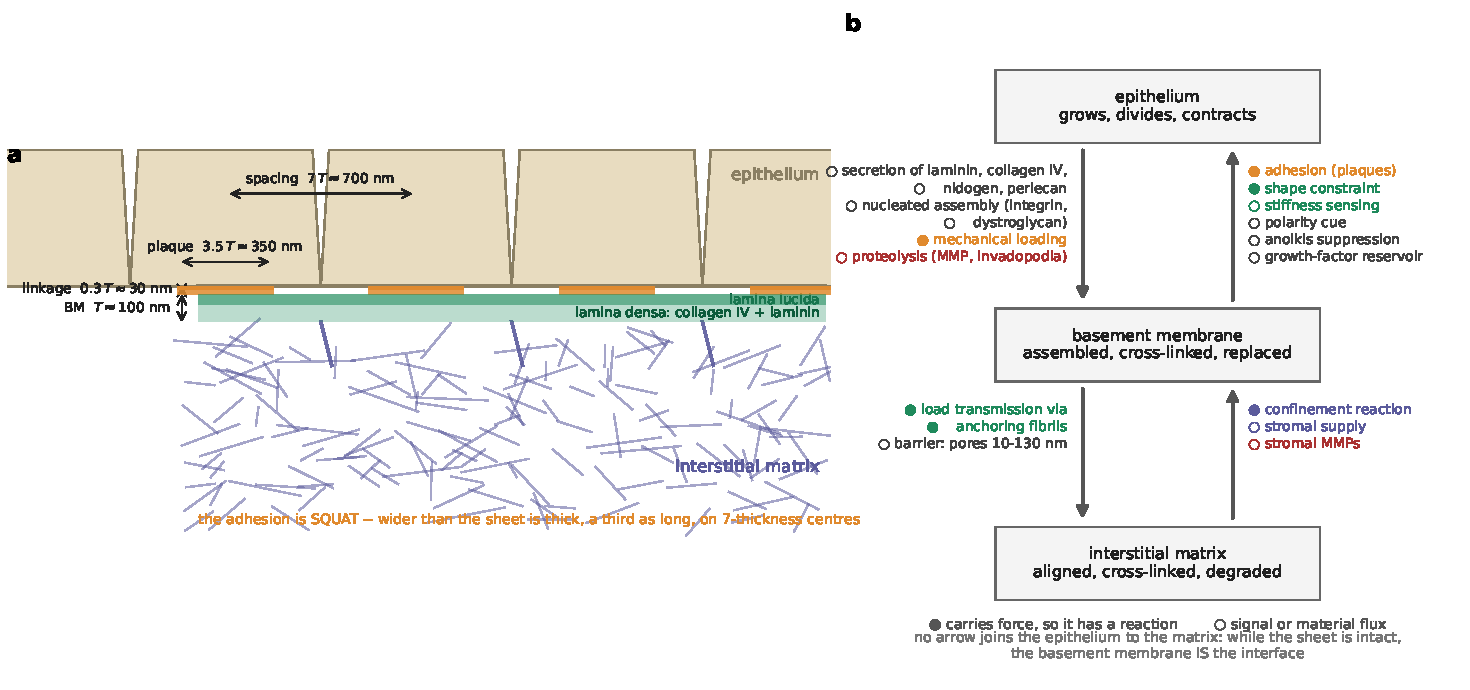
\includegraphics[width=\textwidth]{fig_spheroid_bm_ecm.pdf}
\caption{(a) The three entities in section, at the proportions the literature measures rather than the
ones that are convenient: the adhesion is a squat plaque, not a thread, and the sheet is thin against
its own spacing. (b) Every operator, in the direction it acts. Filled bullets carry a force and must
therefore have a reaction; open bullets carry a signal or a material flux. There is no arrow between
the epithelium and the matrix.}
\end{figure}

\section*{2.\; Equations and symbols}

Each equation below belongs to one arrow of Fig.~1b. The companion notes carry the mechanics of each
entity; this note carries what passes \emph{between} them.

\textbf{Mass, not just mechanics.} The sheet carries an areal density $\rho$ of collagen~IV produced by
the epithelium and removed by proteolysis, on a surface whose area is growing:
%
\begin{equation}
\frac{\mathrm D\rho}{\mathrm Dt}
=\underbrace{s(\mathbf x,t)}_{\text{secretion}}
-\underbrace{\frac{\rho}{\tau_{\rm bm}}}_{\text{turnover}}
-\underbrace{\rho\frac{\dot A}{A}}_{\text{dilution}},
\qquad
s^\ast=\rho\Bigl(\frac1{\tau_{\rm bm}}+\frac{\dot A}{A}\Bigr),
\qquad \tau_{\rm bm}=\frac{t_{1/2}}{\ln2}\approx4\text{--}14\ \text{h}.
\label{eq:bmmass}
\end{equation}
%
The two removal terms are the same size here --- a spheroid tripling its radius over a day has
$\dot A/A\sim10^{-1}\,$h$^{-1}$ against $1/\tau_{\rm bm}\sim10^{-1}\,$h$^{-1}$. Turnover is not a
correction to growth; it is the same size as growth, which is why the sheet can accommodate it at all.

\textbf{A nonlinear sheet.} A single Young's modulus is wrong by construction: the same membrane reads
$\sim\!0.4$ MPa at low strain and $\sim\!3$ MPa at high \cite{candiello2007}, and a growing spheroid
takes it across that range:
%
\begin{equation}
E(\lambda)=E_0\bigl[1+\beta(\lambda-1)\bigr],\qquad
\lambda=\sigma_{\max}(\mathbf F),\qquad
\frac{E_{\rm bm}}{E_{\rm ecm}}\in[10,100].
\label{eq:bmstiff}
\end{equation}
%
\textbf{MPa is not a quantity this box has} --- it is dimensionless and the stroma's modulus is the
number $15$ --- so the falsifiable forms are the two ratios and never the pascals.

\textbf{Adhesion, with its reaction and with slip.} A plaque is two-sided: whatever force it applies to
the sheet it applies equally and oppositely to the cell, which a replayed epithelium discards. And the
sheet is not pinned --- it \emph{slides} --- so the tangential law is friction against relative
velocity and not a spring to a frozen direction:
%
\begin{align}
\mathbf f^{\rm adh}_p&=\kappa_n(\ell_p-\ell_0)\hat{\mathbf n}_p
 -\xi\bigl(\mathbf v_{\rm bm}-\mathbf v_{\rm epi}\bigr)_{\parallel},
&\mathbf f^{\rm epi}_p&=-\mathbf f^{\rm adh}_p,
\label{eq:adh}\\
n_p&=\Sigma^{-2}\ \text{plaques per unit area},\quad \Sigma\approx7T,
&\ell_0&\approx0.3\,T .
\label{eq:plaque}
\end{align}
%
$\ell_0$ is a material property and not a tuning constant: it is what sets the standoff.

\textbf{Sheet to stroma.} Anchoring fibrils \cite{keene1987} load the stroma \emph{through} the sheet,
which is also what lets a stiff sheet spread a local epithelial push over a soft matrix:
%
\begin{equation}
\mathbf t=k_a\bigl(\mathbf x_{\rm ecm}-\mathbf x_{\rm bm}\bigr)\ \text{on anchored points},
\qquad
\mathbf f^{\rm bm}=-\!\!\sum_{\rm anchors}\!\mathbf t .
\label{eq:anchor}
\end{equation}
%
The barrier is geometric rather than mechanical: pores of $10$--$130$ nm pass solutes, stop cells
\cite{yurchenco2011}, and are what a proteolytic operator has to open before anything crosses.

\textbf{The matrix pushes back on the cell cycle.} The force the stroma returns, collected by direction
and divided by the area each direction covers, is a pressure; a cell facing a stressed matrix grows
more slowly, which is what a spheroid grown under a measured external stress does
\cite{helmlinger1997,montel2011}:
%
\begin{equation}
g=f+\frac{1-f}{1+(P/p_{1/2})^n},
\qquad s_{\rm now}\leftarrow s_{\rm prev}\bigl(1+g\,(f_{\rm grow}-1)\bigr).
\label{eq:gate}
\end{equation}
%
Because it is the growth \emph{rate} that is slowed and not the size directly, a small difference
compounds over hundreds of frames --- which is how a modest difference in stress between one direction
and another becomes a difference in shape.

\smallskip
{\small\begin{tabular}{@{}llp{8.4cm}@{}}\toprule
symbol & is & of what\\\midrule
$\rho$, $\tau_{\rm bm}$, $s$ & areal density, turnover time, secretion & of collagen~IV on the sheet,
  Eq.~\eqref{eq:bmmass}\\
$A$, $\dot A/A$ & sheet area, its relative growth rate & the dilution term; the SAME size as turnover\\
$E_0$, $\beta$, $\lambda$ & low-strain modulus, stiffening, principal stretch & of the sheet,
  Eq.~\eqref{eq:bmstiff}; report RATIOS, never MPa\\
$T$, $\Sigma$, $\ell_0$ & thickness, plaque spacing, linkage rest length & $\Sigma\approx7T$,
  $\ell_0\approx0.3T$; $T$ never appears as geometry\\
$\kappa_n$, $\xi$ & plaque normal stiffness, tangential friction & against RELATIVE velocity ---
  $\xi$ is what lets the sheet stay attached while the tissue slides\\
$k_a$ & fibril stiffness & sheet to stroma, Eq.~\eqref{eq:anchor}\\
$P$, $p_{1/2}$, $n$, $f$ & matrix pressure, gate half-point, sharpness, floor & Eq.~\eqref{eq:gate};
  $f\le g\le1$ multiplies the growth RATE\\
\bottomrule\end{tabular}}

\section*{3.\; The Plexus2 container}

\textbf{Two structural claims, and both differ from what the archived line built.} An adhesion is not
a body and a fibril is not a particle: each is a \emph{relation between two entities}, which in
Plexus2 is an edge set carrying \code{.pre} and \code{.post} index buffers rather than a set of nodes
with positions. Writing the hemidesmosome as an edge set is what makes its reaction automatic --- one
operator returns a delta to both endpoints, so the force the sheet feels and the force the cell feels
cannot get out of step. The archived line made the adhesion first a field on the membrane and then a
column of MPM particles, and both lost the reaction.

\begin{center}\small
\begin{tabular}{@{}llll@{}}\toprule
\textbf{set} & \textbf{kind} & \textbf{one element is} & \textbf{state it carries}\\\midrule
\code{spheroid}     & node, depth 0 & the organ & centroid, cell count\\
\quad\code{cell}    & node, depth 1 & one epithelial cell & $A,P,V$ and targets, age, $\rho_f$\\
\quad\code{vertex}  & node, depth 1 & a corner of the apical mesh & \code{pos}\\
\quad\code{junction}& \textbf{edge} $\subseteq$ \code{vertex}$^2$ & a cell--cell contact & $n_e$,
  $\ell_e$\\\midrule
\code{bm}           & node on a surface mesh & a patch of membrane & \code{pos}, $\mathbf F$, $\rho$,
  age, \code{occ}\\
\code{bm\_face}     & \textbf{hyperedge} $\subseteq$ \code{bm}$^3$ & a triangle of membrane &
  $\mathbf D_m^{-1}$, $\mathbf C_0$, $A^0$, $Y_2$\\
\code{plaque}       & \textbf{edge} \code{cell}$\to$\code{bm} & one hemidesmosome & $\ell_0$, load,
  bound\\
\code{fibril}       & \textbf{edge} \code{bm}$\to$\code{mpm\_particle} & one anchoring fibril & rest
  length, load\\\midrule
\code{mpm\_particle}& node, depth 1 & a patch of \emph{stroma only} & \code{pos}, $\mathbf F$, fibre
  direction\\
\code{mpm\_grid}    & \textbf{field} & the stroma's momentum & mass, momentum\\
\code{protease}     & \textbf{field} & MMP concentration & scalar, diffusing\\
\bottomrule\end{tabular}
\end{center}

\begin{center}\footnotesize
\begin{tabular}{@{}lllp{4.2cm}p{3.0cm}@{}}\toprule
\textbf{operator} & \textbf{kind} & \textbf{acts on} & \textbf{mechanism} & \textbf{where its gates
are}\\\midrule
\multicolumn{5}{@{}l}{\textit{epithelium}}\\
\op{grow\_3d}, \op{divide\_3d} & Divide & \code{cell} & volume growth and cytokinesis
  \cite{honda2004,okuda2013} & \op{00}; \code{note\_junction}\\
\op{shape\_energy\_3d} & Lateral & \code{junction} & vertex-model force balance \cite{okuda2018} &
  \op{00}\\
\op{medioapical\_myosin}, \op{junction\_myosin}, \op{cytokinetic\_ring} & Lateral, Structural &
  \code{cell}, \code{junction} & two myosin pools and the ring & \code{note\_junction} J1--J11\\
\multicolumn{5}{@{}l}{\textit{epithelium $\to$ basement membrane}}\\
\op{bm\_secrete}, \op{bm\_degrade} & Divide, Die & \code{bm\_face} & Eq.~\eqref{eq:bmmass}
  \cite{matsubayashi2020,kelley2019} & \code{note\_sheet} G24--G26, G19--G23\\
\op{bm\_stiffness}, \op{bm\_elastic} & Lateral & \code{bm\_face} & Eq.~\eqref{eq:bmstiff} &
  \code{note\_sheet} G1--G8\\
\multicolumn{5}{@{}l}{\textit{basement membrane $\leftrightarrow$ epithelium}}\\
\op{plaque\_seed}, \op{plaque\_pull}, \op{plaque\_rupture} & Rewire, Lateral & \code{plaque} &
  Eqs.~\eqref{eq:adh}--\eqref{eq:plaque}, \emph{with the reaction} \cite{kanchanawong2010} &
  \code{note\_sheet} G9--G13\\
\multicolumn{5}{@{}l}{\textit{basement membrane $\leftrightarrow$ matrix}}\\
\op{fibril\_seed}, \op{fibril\_pull} & Rewire, Lateral & \code{fibril} & Eq.~\eqref{eq:anchor}
  \cite{keene1987} & open\\
\op{mesh\_contact} & Lateral & \code{contact} & particle-to-surface, both endpoints in one call &
  \code{note\_surface} S1--S16\\
\op{bm\_barrier} & Exchange & \code{bm\_face}, fields & pores pass solutes, stop cells
  \cite{yurchenco2011} & open\\
\multicolumn{5}{@{}l}{\textit{matrix}}\\
\op{seed\_ecm}, \op{mpm\_*}, \op{ecm\_stress} & Seed, Exchange, Lateral & \code{mpm\_particle} &
  MLS-MPM \cite{sulsky1994,hu2018} & \code{note\_fibre} F1--F16\\
\op{ecm\_growth\_gate\_3d} & Lateral & \code{cell} & Eq.~\eqref{eq:gate}
  \cite{helmlinger1997,montel2011} & \op{58}; open\\
\bottomrule\end{tabular}
\end{center}

\textbf{One schedule, split at exactly one place.} Anything carrying a force runs inside the substep
block, at the stroma's rate; anything changing topology or mass runs once per frame, because a set
whose membership changed mid-substep would be integrated against two different index sets in one step:
%
\begin{align*}
\text{frame }(\Delta t=1):\ \ &\op{cell\_geometry\_3d}\to\op{grow\_3d}\to\op{bm\_growth\_gate}
 \to\op{medioapical\_myosin}\to\op{junction\_myosin}\\
&\to\op{shape\_energy\_3d}\to\op{reconnect\_t1\_3d}\to\op{divide\_3d}\to\op{cytokinetic\_ring}
 \to\op{junction\_myosin\_sync}\\
&\to\op{bm\_refine}\to\op{bm\_secrete}\to\op{bm\_degrade}\to\op{plaque\_seed}\to
 \op{plaque\_rupture}\\[3pt]
\text{substep }(\Delta t_{\rm sub}=\Delta t/8):\ \
&\op{bm\_stiffness}\to\op{bm\_elastic}\to\op{plaque\_pull}\to\op{fibril\_pull}\\
&\to\op{mpm\_strain}\to\op{mpm\_scatter}\to\op{mpm\_grid\_update}\to\op{mpm\_gather}
\end{align*}

\textbf{Four rules, each buying something specific.} \emph{The membrane never enters the grid} --- it
is $\sim\!100$ nm on a $\sim\!200\,\mu$m spheroid, so resolving it as MPM material needs a $3500^3$
lattice; as a surface mesh it costs what the epithelium costs and $\Delta x$ is set by the stroma
alone. \emph{The epithelium stays out of the substep block} --- it is overdamped and massless, so it
does not need the matrix's CFL step, and putting its relaxation inside would multiply its cost by
eight and change nothing. \emph{The sheet is massless too}, so its stiffness costs drag rather than
substeps: the bound is $\Delta t\,(zk_b+\kappa)/\gamma<2$, a rate and not a wave speed, and the
$10$--$100$ stiffness ratio is paid for with $\gamma$. \emph{Particles go on the shell that carries
stress, not on the box} --- the far field is quiescent, and filling the box at a usable density costs a
million particles.

\textbf{And one thing this deletes.} \op{cell\_to\_ecm} and \op{cell\_exclude\_3d} go, because while
the sheet is intact the basement membrane \emph{is} the interface (\S1). MPM fibres also stop being
asked to act as ropes, which \code{note\_fibre} measured they cannot.

\section*{4.\; Gates}

A gate is a number with a threshold decided \emph{before} the run and a stated consequence if it
fails. The per-entity gates live in the companion notes and are indexed in \S3; this table is the
\emph{system} level --- what has to be true of the assembled model, and which arrows are not yet built.

\smallskip
{\scriptsize\setlength{\tabcolsep}{4pt}
\begin{tabularx}{\textwidth}{@{}llLl@{}}\toprule
& \textbf{gate} & \textbf{threshold} & \textbf{measured}\\\midrule
\multicolumn{4}{@{}l}{\textit{the epithelium is unchanged by everything attached to it} (\op{00} is
the reference)}\\
B1 & cells, radius, aspect, T1 rate of the bare tissue & the numbers every later run must reproduce &
     \pass{$200\to6076$}, $\times$\pass{3.56}, \pass{1.021}, \pass{0.0089}/cell/frame\\
B2 & adding per-junction myosin at $m_e\equiv1$ changes nothing & bit-identical &
     \pass{bit-identical}\\
\multicolumn{4}{@{}l}{\textit{each arrow carries its reaction}}\\
B3 & epithelium $\to$ matrix, momentum residual & $<10^{-6}$ & \pass{1.2e-7} max, \pass{1.5e-8}
     median (\code{note\_surface} S5)\\
B4 & cell $\leftrightarrow$ sheet, as bookkeeping and as motion & $<10\varepsilon_{64}$; drift
     $<10^{-12}$ & \pass{1.4e-16}, \pass{4.4e-15} (\code{note\_sheet} G9, G10)\\
B5 & sheet $\to$ stroma: the stroma is loaded THROUGH the sheet & displacement with the sheet present
     vs absent & \fail{not built} --- \op{fibril\_pull} is the missing arrow\\
\multicolumn{4}{@{}l}{\textit{the middle entity does what a membrane does}}\\
B6 & the sheet reports its own deformation & $>0.95$ of the geometric stretch &
     \pass{0.9935} as a surface; \fail{0.13} as MPM material (run 130)\\
B7 & $\rho$ held flat while $A$ triples & within $10\%$ & \fail{$1/11.1$} with no secretion
     (\code{note\_sheet} G24)\\
B8 & the standoff is the linkage's rest length & $\ell/\ell_0\in[0.9,1.1]$ & \fail{3.43}
     (\code{note\_sheet} G12)\\
\multicolumn{4}{@{}l}{\textit{the coupling is mutual}}\\
B9 & the tissue feels the matrix: shape differs from the free control & any separation &
     \fail{one-way} --- the reaction is computed, recorded and dropped\\
B10& the growth gate changes the shape it is given & oblateness against the unconfined run &
     \pass{1.43} grown vs \pass{1.41} pressed (\op{58}, \op{48})\\
\bottomrule\end{tabularx}}
\smallskip

\textbf{One convention makes these mean what they say.} \textbf{A reaction is measured on its own force
pair}, inside the substep and before any drive is added; with the drive in the sum it stops being a
statement about the reaction. That is why B3 and B4 are separate rows with different thresholds: B3 is
float32 through a grid, B4 is float64 on an explicit edge.

\textbf{What the gates license.} The epithelium is reproducible on its own and nothing attached to it
has moved it (B1, B2); every arrow that has been built returns its reaction to machine precision (B3,
B4); the sheet, as a surface, reports the deformation it is given (B6); and the growth gate can produce
a shape that pressing produces too, which is the one place the matrix has been shown to change the
tissue (B10). \textbf{What they do not license} is the assembled model: B5 is not built, B7 and B8 fail
on the sheet's own testbench, and B9 is the architecture --- the tissue is a replay, so it drives and
is never driven. Until B9 passes, the stroma's modulus is very nearly a free parameter: the tissue never
feels the matrix, and the growth gate normalises the pressure map to its own late-run median, so a
softer stroma changes the substep it needs and not the shape that comes out. That is the clearest
statement of what one-way coupling costs, and \op{mesh\_contact} returning \code{vertex\_force} to a
live epithelium is the run that ends it.

\textbf{What sixty-six archived runs settled, and it is four things.} Runs \op{91}--\op{164} asked
where the sheet sits and what holds it there, and they answer that question and no other. The standoff
is a \emph{tracking lag}, $\delta-\dot R\Delta t\gamma/\kappa$, and not a force balance, which two
fibre lengths differing fourfold confirmed to $3\times10^{-5}$ box units. A force routed through the
grid leaves the sheet carrying $100\%$ of its true stretch while the same force integrated by the
engine leaves it carrying $13\%$ (B6). An MPM fibre cannot act as a rope, because $\mathbf F$ is
advected by the grid's velocity gradient and never measures the distance between two particles. And
every MPM body in the prototype silently carried the \emph{parent} set's modulus, so a membrane
declaring $E=400$ ran at the stroma's $15$ until each body was given its own parent --- which is why
run 146 came back bit-identical to run 144 at ten times the stiffness. None of the four is a model
derived from what a basement membrane \emph{is}; that is what \code{note\_sheet} builds.

\section*{5.\; References}

{\small
\begin{thebibliography}{99}\setlength{\itemsep}{0pt}
\bibitem{sulsky1994} Sulsky, D., Chen, Z., Schreyer, H.L. (1994) A particle method for
history-dependent materials. \emph{Comput. Methods Appl. Mech. Eng.} \textbf{118}:179--196.
\bibitem{hu2018} Hu, Y. \emph{et al.} (2018) A moving least squares material point method with
displacement discontinuity and two-way rigid body coupling. \emph{ACM Trans. Graph.} \textbf{37}(4):150.
\bibitem{honda2004} Honda, H., Tanemura, M., Nagai, T. (2004) A three-dimensional vertex dynamics cell
model of space-filling polyhedra. \emph{J. Theor. Biol.} \textbf{226}(4):439--453.
\bibitem{okuda2013} Okuda, S., Inoue, Y., Eiraku, M., Sasai, Y., Adachi, T. (2013) Reversible network
reconnection model for simulating large deformation in dynamic tissue morphogenesis.
\emph{Biomech. Model. Mechanobiol.} \textbf{12}(4):627--644.
\bibitem{okuda2018} Okuda, S., Miura, T., Inoue, Y., Adachi, T., Eiraku, M. (2018) Combining Turing
and 3D vertex models reproduces autonomous multicellular morphogenesis. \emph{Sci. Rep.} \textbf{8}:2386.
\bibitem{helmlinger1997} Helmlinger, G., Netti, P.A., Lichtenbeld, H.C., Melder, R.J., Jain, R.K.
(1997) Solid stress inhibits the growth of multicellular tumor spheroids. \emph{Nat. Biotechnol.}
\textbf{15}(8):778--783.
\bibitem{montel2011} Montel, F. \emph{et al.} (2011) Stress clamp experiments on multicellular tumor
spheroids. \emph{Phys. Rev. Lett.} \textbf{107}:188102.
\bibitem{yurchenco2011} Yurchenco, P.D. (2011) Basement membranes: cell scaffoldings and signaling
platforms. \emph{Cold Spring Harb. Perspect. Biol.} \textbf{3}(2):a004911.
\bibitem{candiello2007} Candiello, J. \emph{et al.} (2007) Biomechanical properties of native basement
membranes. \emph{FEBS J.} \textbf{274}(11):2897--2908.
\bibitem{matsubayashi2020} Matsubayashi, Y. \emph{et al.} (2020) Rapid homeostatic turnover of
embryonic ECM during tissue morphogenesis. \emph{Dev. Cell} \textbf{54}(1):33--42.
\bibitem{changede2017} Changede, R., Sheetz, M. (2017) Integrin and cadherin clusters: a robust
way to organize adhesions for cell mechanics. \emph{BioEssays} \textbf{39}(1):1600123. --- nascent
adhesions are $\sim\!100$ nm and contain $\sim\!50$ integrins; large adhesions are loose aggregates of
such clusters.
\bibitem{nanoclusters2025} \emph{Differential spatial regulation and activation of integrin
nanoclusters inside focal adhesions.} eLife reviewed preprint 105270. --- STORM: nanocluster median
size $35$--$40$ nm, centre-to-centre $\sim\!555$ nm, spacing set cell-intrinsically. Cited as a
preprint.
\bibitem{kanchanawong2010} Kanchanawong, P. \emph{et al.} (2010) Nanoscale architecture of
integrin-based cell adhesions. \emph{Nature} \textbf{468}:580--584.
\bibitem{keene1987} Keene, D.R., Sakai, L.Y., Lunstrum, G.P., Morris, N.P., Burgeson, R.E. (1987)
Type VII collagen forms an extended network of anchoring fibrils. \emph{J. Cell Biol.}
\textbf{104}(3):611--621.
\bibitem{kelley2019} Kelley, L.C. \emph{et al.} (2019) Adaptive F-actin polymerization and localized
ATP production drive basement membrane invasion in the absence of MMPs. \emph{Dev. Cell}
\textbf{48}(3):313--328.
\end{thebibliography}}

\end{document}
